\documentclass[11pt]{article}
\usepackage[italian]{babel}
\usepackage{geometry}
\usepackage{graphicx} 
\geometry{a4paper} 
\usepackage{listings} % necessario per inclusione codice sorgente
\usepackage{mips}
\usepackage{color} % syntax highlighting
\usepackage{url}
% qualsiasi altro package necessario può essere aggiunto qui ...

% definizione dei colori  
\definecolor{dkgreen}{rgb}{0,0.6,0}
\definecolor{gray}{rgb}{0.5,0.5,0.5}
\definecolor{mauve}{rgb}{0.58,0,0.82}

% definizione set keywords e parametri generici
\lstset{ %
  language=[mips]Assembler,       % the language of the code
  basicstyle=\footnotesize,       % the size of the fonts that are used for the code
  numbers=left,                   % where to put the line-numbers
  numberstyle=\tiny\color{gray},  % the style that is used for the line-numbers
  stepnumber=1,                   % the step between two line-numbers. If it's 1, each line 
                                  % will be numbered
  numbersep=5pt,                  % how far the line-numbers are from the code
  backgroundcolor=\color{white},  % choose the background color. You must add \usepackage{color}
  showspaces=false,               % show spaces adding particular underscores
  showstringspaces=false,         % underline spaces within strings
  showtabs=false,                 % show tabs within strings adding particular underscores
  frame=single,                   % adds a frame around the code
  rulecolor=\color{black},        % if not set, the frame-color may be changed on line-breaks within not-black text (e.g. commens (green here))
  tabsize=4,                      % sets default tabsize to 2 spaces
  captionpos=b,                   % sets the caption-position to bottom
  breaklines=true,                % sets automatic line breaking
  breakatwhitespace=false,        % sets if automatic breaks should only happen at whitespace
  title=\lstname,                 % show the filename of files included with \lstinputlisting;
                                  % also try caption instead of title
  keywordstyle=\color{blue},          % keyword style
  commentstyle=\color{dkgreen},       % comment style
  stringstyle=\color{mauve},         % string literal style
  escapeinside={\%*}{*)},            % if you want to add a comment within your code
  morekeywords={*,...}               % if you want to add more keywords to the set
}

\pdfinfo{
   /Author (Pinco Pallino)
   /Title  (Specifica del Progetto di Laboratorio - Architetture 2 - Turno A)
  % /Title  (Specifica del Progetto di Laboratorio - Architetture 1 - Turno B)
}

\title{Specifica del Progetto di Laboratorio \\ Architettura degli Elaboratori I}
%\title{Specifica del Progetto di Laboratorio \\ Architettura degli Elaboratori II}
%\title{Relazione del Progetto di Laboratorio \\ Architettura degli Elaboratori I}



% \thanks{} e le date al suo interno vanno incluse solo in fase di consegna
\author{Pinco Pallino\thanks{Progetto approvato il 21/01/2016, consegnato il 27/03/2016}\\ matricola: 12345, Turno: A\\ \url{pinco.pallino@studenti.unimi.it}}

\date{} % lasciare vuota

\begin{document}
\maketitle

% struttura e numero delle sezioni è a discrezione dello studente
% per la lunghezza complessiva del documento si tengano conto di queste linee guida
% specifica: non più di una pagina
% relazione (solo per Architetture 1): non più di 10 pagine

\section{Titolo prima sezione}

\begin{figure}[!htpb]
\centering
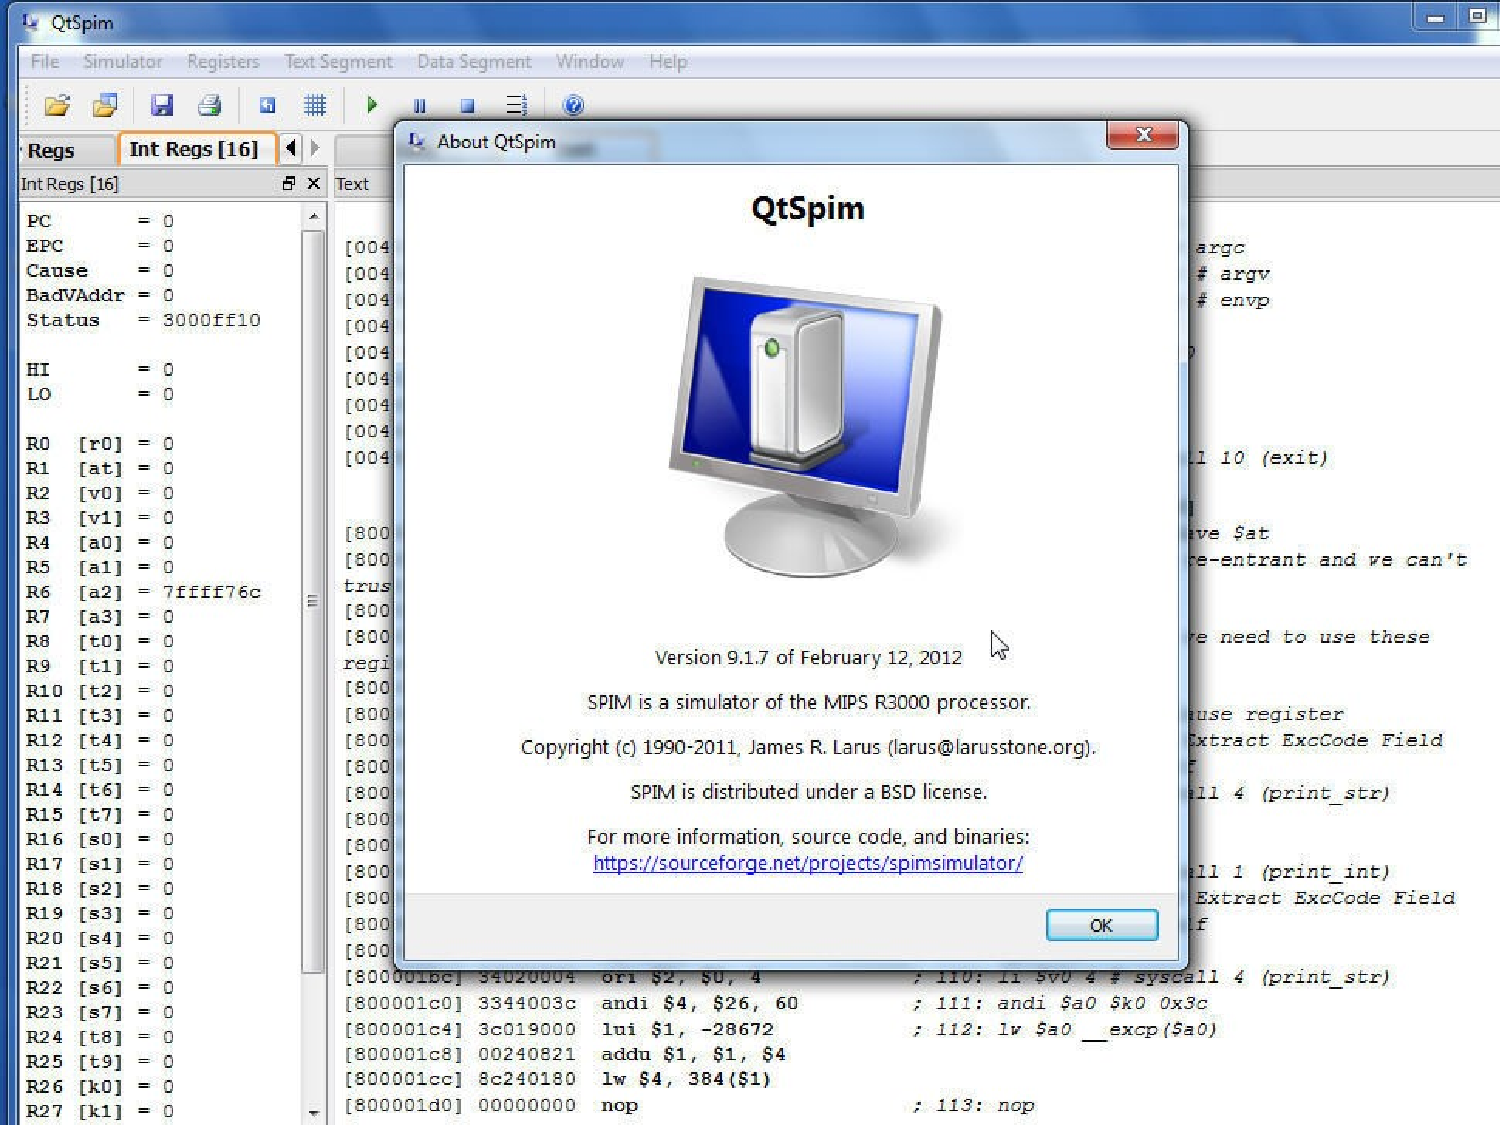
\includegraphics[width=0.3\columnwidth]{immagini/esempio_immagine_spim}
\caption{Screenshot del simulatore QtSpim}
\label{fig:qtspim}
\end{figure}

\subsection{Sottosezione}

\begin{figure}[!htpb]
\centering
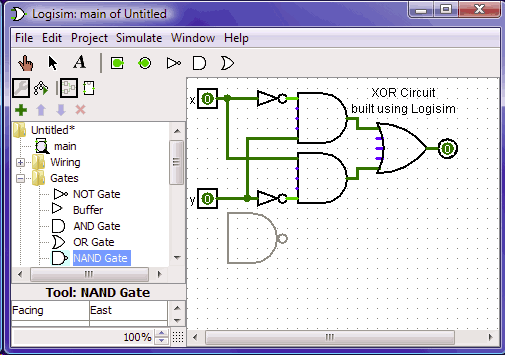
\includegraphics[width=0.3\columnwidth]{immagini/esempio_immagine_logisim}
\caption{Screenshot del simulatore Logisim}
\label{fig:logisim}
\end{figure}

\section{Titolo seconda sezione}
Gli strumenti software utilizzati nel laboratorio di Architetture sono Logisim per Architetture 1 (si veda Figura~\ref{fig:logisim}) e QtSpim per Architetture~2 (si veda Figura~\ref{fig:qtspim}).

\section{Listati Assembly}
Per inserire codice Assembly MIPS nella relazione possiamo utilizzare il comando \textit{listinputlisting}:\\
\lstinputlisting{esempio_codice_assembly.asm} 
Esso si utilizza con la seguente sintassi:
\begin{verbatim} 
 \lstinputlisting{esempio_codice_assembly.asm} 
\end{verbatim} 
Listinputlisting include nel documento il contenuto del file \textit{esempio\_codice\_assembly.asm} dopo averlo formattato (evidenziandone sintassi e parole chiave) ed aver numerato le righe del sorgente in modo da rendere pi\`u semplice il riferimento ad esse nel testo della relazione.

\end{document}